\chapter{Manuales de uso e instalaci'on}

\section{Dependencias}
Las dependencias del sistema pueden clasificarse en dos tipos:\\
%Compilación
\textbf{Compilaci'on} 
\\
Para compilar el programa es necesario tener instalados los siguientes programas:
\begin{itemize}
 \item g+
  \item fortran
  \item Biblioteca mysqlconnector para C  
\end{itemize}

%Operación
\textbf{Operaci'on} 

\begin{itemize}
 \item Paquete de programas grads version 2.0.a7.1 o superior.
  \item Apache tomcat 7 o superior o algún otro servidor web que soporte JSF y PrimeFaces.
  \item Convert. Este programa es usado para transformar las im'agenes de lluvias en jpeg.
\end{itemize}

\section{Instalaci'on}
%uso del instalador del programa en C++ / Fortran
Se gener'o un instalador en bash que permite configurar el entorno y verificar las dependencias para poder compilar
el programa.
%ínstalación de la página web
El desarrollo de la página web se realiz'o usando Netbeans 7.0. La instalaci'on de la p'agina en el servidor Tomcat requiere que
simplemente se copie el archivo AsimilacionLluvias.war en la carpeta de aplicaciones de Tomcat. Posteriormente el servidor 
desempaquetar'a el archivo y la apliaci'on podr'a ser accedida.

La aplicaci'on web usa internamente el programa en C++/Fortran para realizar los c'alculos num'ericos. Por lo que hay que copiar
la aplicaci'on num'erica en la direcci'on AsimilacionLluvias/web/Asimilacion y adem'as se deben poner los permisos adecuados para
que el servidor web pueda ejecutar la apliaci'on.

\section{Preparaci'on de la Base de Datos}
\subsubsection*{Archivos separados por comas}
El primer paso es crear los archivos csv que se subir'an a la base de datos. Existen tres tipos de archivos que pueden ser usados: \\

\textbf{Archivo de Cuencas} \\
'Este archivo es sumamente sencillo pues consta de un identificador num'erico 'unico y el nombre de la cuenca. \\

\textbf{Archivo de lecuras de estaciones en tierra}  \\
'Este archivo consta de los siguientes campos: Identificador 'unico, identificador de la estaci'on que realiz'o la lectura, precipitaci'on
y fecha en el formato YYYY-MM-DD HH:00:00. \\

\textbf{Archivo de definici'on de estaciones} \\
El archivo que define las estaciones est'a ligado con las cuencas disponibles. Una estaci'on siempre pertenecer'a a una cuenca.
Los campos de 'este archivo son: Identificador de cuenca, Nombre, Longitud, Latitud.\\

\textbf{Archivos que definen la malla artificial}\\
Para poder realizar las interpolaciones y guardar la informaci'on descargada en el sat'elite
se crearon una serie de archivos que definen una malla artificial sobre la República Mexicana.
La Figura 3.1 muestra uno de los 45 archivos archivos de texto que define la malla artificial, 'estos archivos
no deben modificarse. 

\begin{figure}[h!]
 \centering
 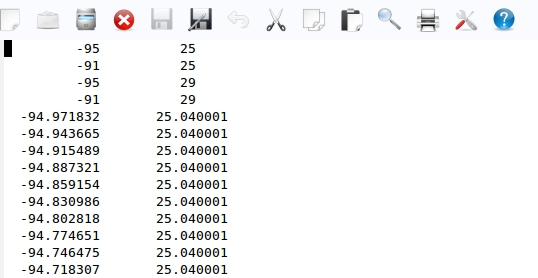
\includegraphics[width=110mm, bb=0 0 538 278]{./imagenes/mallaArificial.jpg}
 % mallaArificial.jpg: 538x278 pixel, 72dpi, 18.98x9.81 cm, bb=0 0 538 278
 \caption{Malla artificial para un sector de la República Mexicana}
\end{figure}

\subsubsection*{Creaci'on de la base de datos y carga de contenido}
%Correr los scripts
Es necesario que se posean los privilegios suficientes de administrador para poder realizar el 
proceso de instalaci'on y preparaci'on que se resume en los siguientes pasos:

\begin{enumerate}
 \item Crear la base de datos \textit{Asimilacion1} usando MySQL
  \item Ejecutar el script que crea el esquema de la base de datos con la instrucci'on \\ \texttt{mysql Asimilacion1 < Asimilacion1.1.sql}
  \item Cargar la informaci'on de las cuencas \\ .\textbackslash\texttt{asimilaciondb\_v1 --cuenca Cuenca.csv}
  \item Cargar la informaci'on de las estaciones \\ .\textbackslash\texttt{asimilaciondb\_v1  --station Estaciones.csv }
  \item Cargar la informaci'on de la malla artificial ejecutando el script de carga \\ .\textbackslash\texttt{loadMallaArtificial.sh}
\end{enumerate}


\section{Uso de la aplicaci'on}

El dise\~no del programa contempl'o que la usabilidad de la aplicaci'on fuera igual al de las herramientas de l'inea de comandos de GNU.
De 'esta manera, la curva de aprendizaje del usuario final ser'ia muy reducida especialemente para aquellas personas que est'an 
familiarizados con 'este ambiente de desarrollo. Para lograr 'esto se us'o la biblioteca getopt.h que es estandard de los sistemas UNIX.


\subsubsection*{Programa asimilacion2}
A continuaci'on se lista la serie de opciones de la aplicaci'on
\begin{center}
  \begin{tabular}{|l|p{9cm}|}
  \hline
  - -txt [ARCHIVO] & Sube a la base de datos un archivo de texto del sat'elite y verifica que la 
		      informaci'on no se haya guardado previamente\\ \hline 
  - -txtu [ARCHIVO] & Sube a la base de datos un archivo de texto del sat'elite sin verificar que 
		      la informaci'on sea consistente. Esta opci'on permite la carga m'as r'apida del archivo pero se debe estar seguro que
		      la informaci'on del mismo no est'e previamente en la base de datos\\ \hline
  - -a1 & Indica que se va a calcular el algoritmo Asimilaci'on \\ \hline
  - -rr & Indica que se quiere calcular la primer estimaci'on de lluvia \\ \hline
  - -fpolygon [ARCHIVO] & Indica donde est'a guardado el archivo que define el poligono que se usar'a para realizar el c'alculo \\ \hline
  - -date [YYYY-MM-DD HH] & Indica que fecha y hora se desea calcular \\ \hline
  - -outputdir [ARCHIVO] & Indica en que directorio se va a guardar los productos del c'alculo \\ \hline
  - -asHour [N] & Indica que se usar'an N horas previas para correr Asimilaci'on \\ \hline 
  \end{tabular} 
\end{center}

\subsubsection*{Programa asimilaciondb\_v1}
A continuaci'on se lista la serie de opciones de la aplicaci'on.\\
\begin{center}
  \begin{tabular}{|l|p{9cm}|}
  \hline
  - -station [ARCHIVO] & Sube a la base de datos un archivo que tiene las definiciones de las estaciones.\\ \hline 
  - -cuenca [ARCHIVO] & Sube a la base de datos un archivo csv que tiene definiciones de las cuencas\\ \hline
  - -window [ARCHIVO] & Sube un archivo que define una secci'on de la malla predefinida \\
  \hline 
  \end{tabular} 
\end{center}
